\documentclass[border=4pt]{standalone}
\usepackage{tikz,amsmath}

\begin{document}
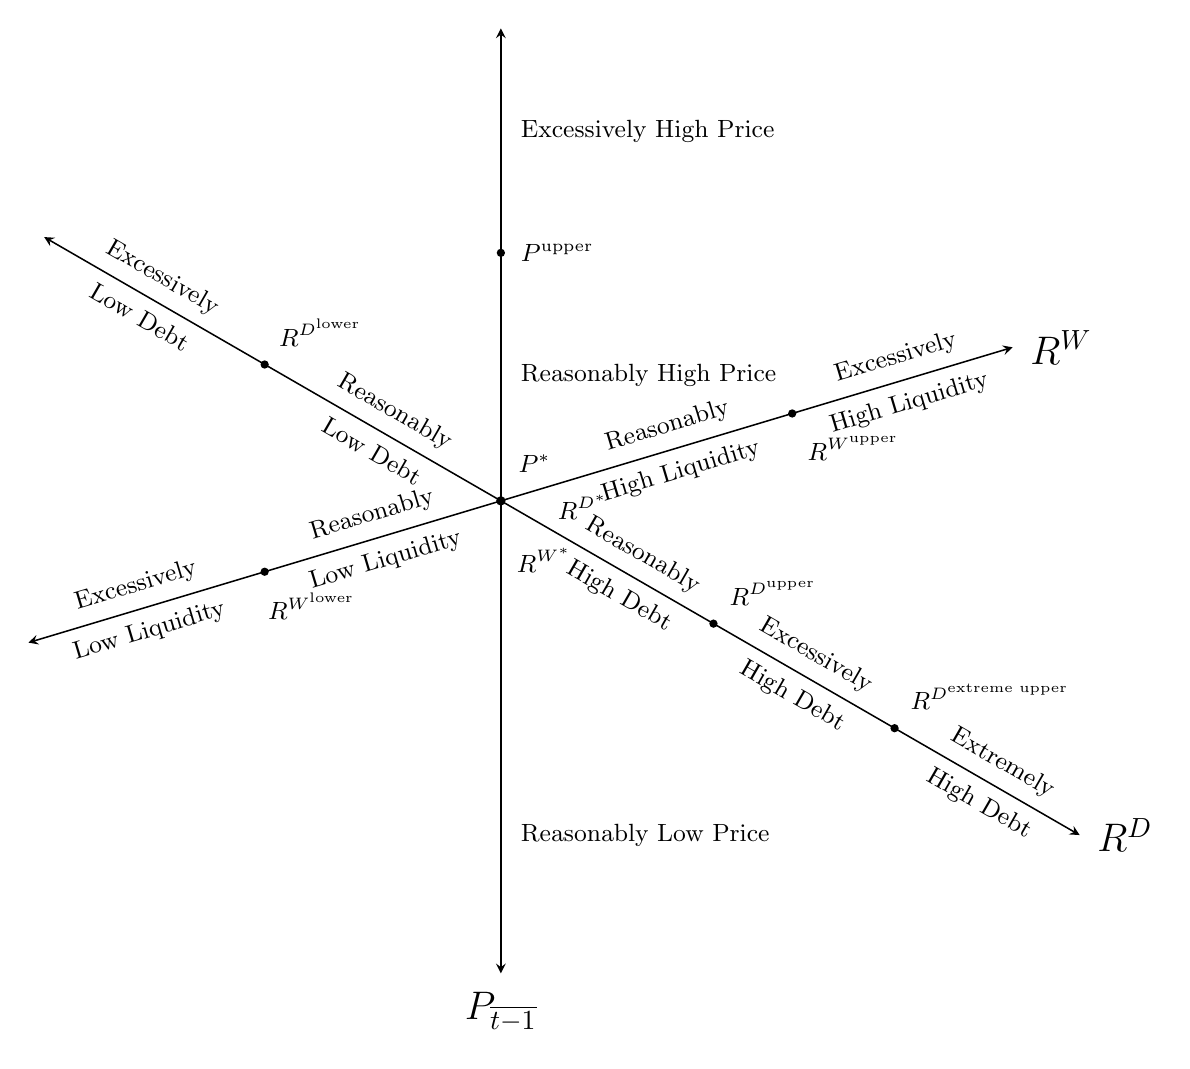
\begin{tikzpicture}[x=1cm,y=1cm,font=\small,>=stealth]
% Native, editable replacement of Position.png. Axes are schematic, not to scale.
% Price and liquidity retain their original categories. Debt has five categories.

% Three axes through the ideal-equilibrium origin.
\draw[<->,line width=0.55pt] (0,-6.0) -- (0,6.0);
\draw[<->,line width=0.55pt] (-6.0,-1.8) -- (6.5,1.95);
\draw[<->,line width=0.55pt] (-5.8,3.35) -- (7.35,-4.244);

% Price axis.
\fill (0,3.15) circle (1.5pt);
\node[anchor=west] at (0.13,3.15) {$P^{\text{upper}}$};
\node[anchor=west] at (0.13,4.7) {Excessively High Price};
\node[anchor=west] at (0.13,1.6) {Reasonably High Price};
\node[anchor=west] at (0.13,-4.25) {Reasonably Low Price};
\node[anchor=north,font=\Large] at (0,-6.12) {$P_{\overline{t-1}}$};

% Liquidity axis and thresholds.
\fill (-3.0,-0.9) circle (1.5pt);
\fill (3.7,1.11) circle (1.5pt);
\node[anchor=north west] at (-3.08,-1.04) {$R^{W^{\text{lower}}}$};
\node[anchor=north west] at (3.77,0.94) {$R^{W^{\text{upper}}}$};
\node[rotate=16.7,anchor=south,yshift=1pt] at (-4.55,-1.365) {Excessively};
\node[rotate=16.7,anchor=north,yshift=-1pt] at (-4.55,-1.365) {Low Liquidity};
\node[rotate=16.7,anchor=south,yshift=1pt] at (-1.55,-0.465) {Reasonably};
\node[rotate=16.7,anchor=north,yshift=-1pt] at (-1.55,-0.465) {Low Liquidity};
\node[rotate=16.7,anchor=south,yshift=1pt] at (2.2,0.66) {Reasonably};
\node[rotate=16.7,anchor=north,yshift=-1pt] at (2.2,0.66) {High Liquidity};
\node[rotate=16.7,anchor=south,yshift=1pt] at (5.1,1.53) {Excessively};
\node[rotate=16.7,anchor=north,yshift=-1pt] at (5.1,1.53) {High Liquidity};
\node[anchor=west,font=\Large] at (6.60,1.95) {$R^W$};

% Debt axis: lower, optimal, upper and extreme thresholds delimit five bands.
\fill (-3.0,1.732) circle (1.5pt);
\fill (2.7,-1.559) circle (1.5pt);
\fill (5.0,-2.887) circle (1.5pt);
\node[anchor=south west] at (-2.94,1.84) {$R^{D^{\text{lower}}}$};
\node[anchor=south west] at (2.78,-1.45) {$R^{D^{\text{upper}}}$};
\node[anchor=south west] at (5.08,-2.78) {$R^{D^{\text{extreme upper}}}$};
\node[rotate=-30,anchor=south,yshift=1pt] at (-4.45,2.569) {Excessively};
\node[rotate=-30,anchor=north,yshift=-1pt] at (-4.45,2.569) {Low Debt};
\node[rotate=-30,anchor=south,yshift=1pt] at (-1.5,0.866) {Reasonably};
\node[rotate=-30,anchor=north,yshift=-1pt] at (-1.5,0.866) {Low Debt};
\node[rotate=-30,anchor=south,yshift=1pt] at (1.65,-0.953) {Reasonably};
\node[rotate=-30,anchor=north,yshift=-1pt] at (1.65,-0.953) {High Debt};
\node[rotate=-30,anchor=south,yshift=1pt] at (3.85,-2.223) {Excessively};
\node[rotate=-30,anchor=north,yshift=-1pt] at (3.85,-2.223) {High Debt};
\node[rotate=-30,anchor=south,yshift=1pt] at (6.22,-3.591) {Extremely};
\node[rotate=-30,anchor=north,yshift=-1pt] at (6.22,-3.591) {High Debt};
\node[anchor=west,font=\Large] at (7.45,-4.244) {$R^D$};

% Shared origin: ideal price, debt and liquidity.
\fill (0,0) circle (1.7pt);
\node[anchor=south west] at (0.10,0.23) {$P^*$};
\node[anchor=west] at (0.60,-0.08) {$R^{D^*}$};
\node[anchor=north west] at (0.08,-0.48) {$R^{W^*}$};
\end{tikzpicture}
\end{document}
